\section{CanOp}
\label{sec_CanOp}
CanOp est le nom qui a été donné au projet de crée une sonde nouvelle génération pour la mine Somaïr au Niger. Cette sonde est composée de 3~pièces.
\begin{itemize}
    \item 2 Sondes de rayonnement Gamma fournissent par la société Geovista
    \item une partie électronique qui inclue une batterie.
    \item Un GPS différentiel fourni par Ophelia
\end{itemize}
Un opérateur utilise cette sonde en connexion avec une tablette pour déterminer ou extraire du minerai.
\subsection{Les sondes Gamma}
\label{ssec_sonde}
Les sondes gamma de cet appareil proviennent de chez Ophelia et sont composées de deux parties.
\begin{figure}

    \begin{subfigure}{1\textwidth}
        \centering
        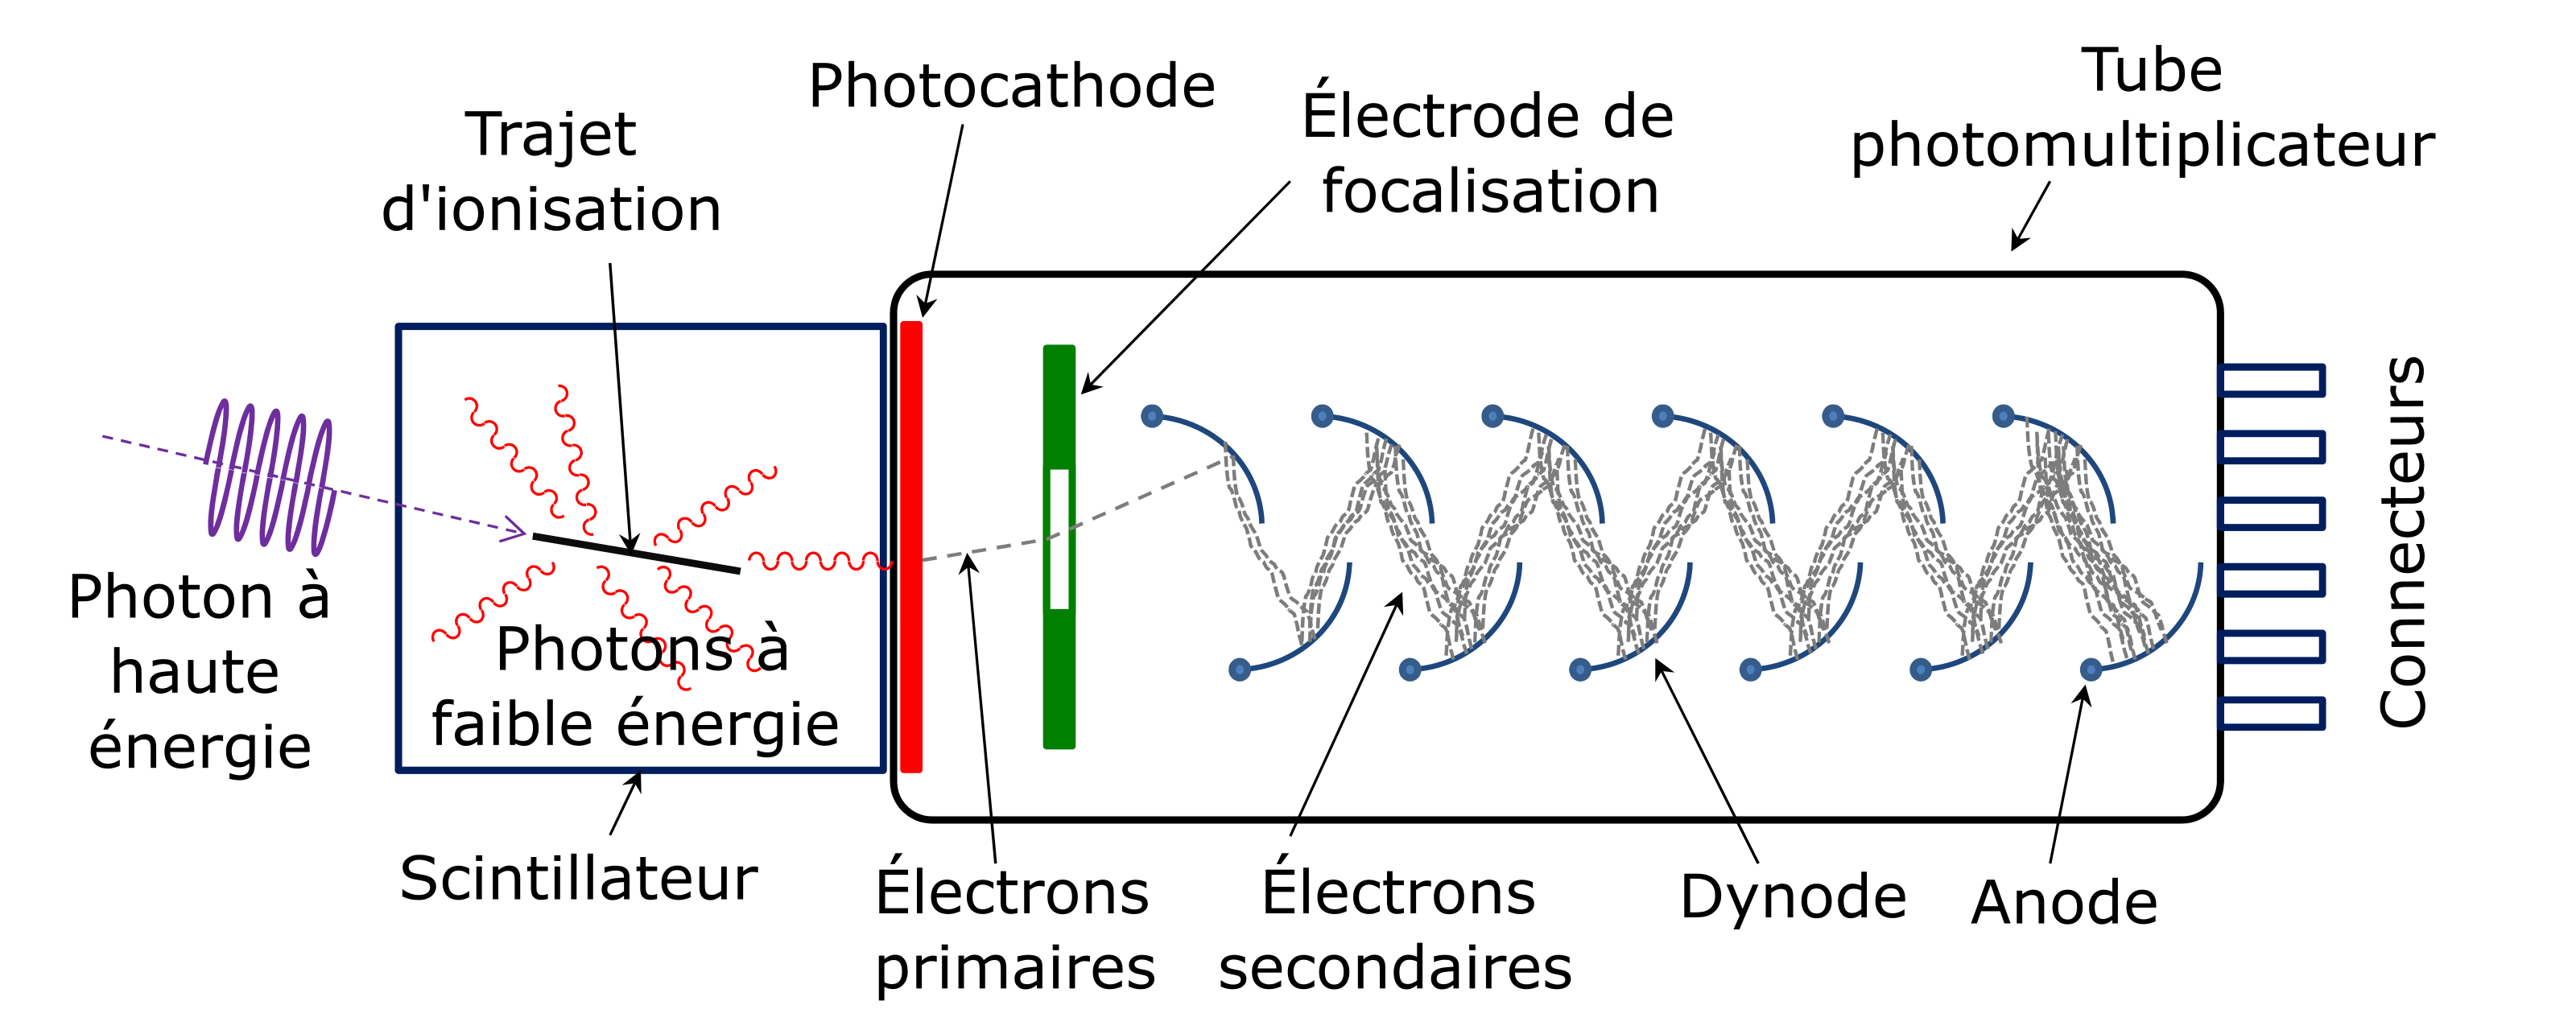
\includegraphics[width=1\textwidth]{she/Photomultiplier_coupled_to_a_scintillator_-_fr.png}
        \caption[Shema d'une sonde gamma NaI]{Schéma d'une sonde gamma NaI. Source~: \href{https://commons.wikimedia.org/wiki/File:Photomultiplier_coupled_to_a_scintillator_-_fr.png}{Qwerty123uiop}, \href{https://creativecommons.org/licenses/by-sa/3.0}{CC BY-SA~3.0}, via Wikimedia Commons}
        \label{fig_detecteur_gamma}
    \end{subfigure}
    \begin{subfigure}[t]{0.5\textwidth}
        \centering
        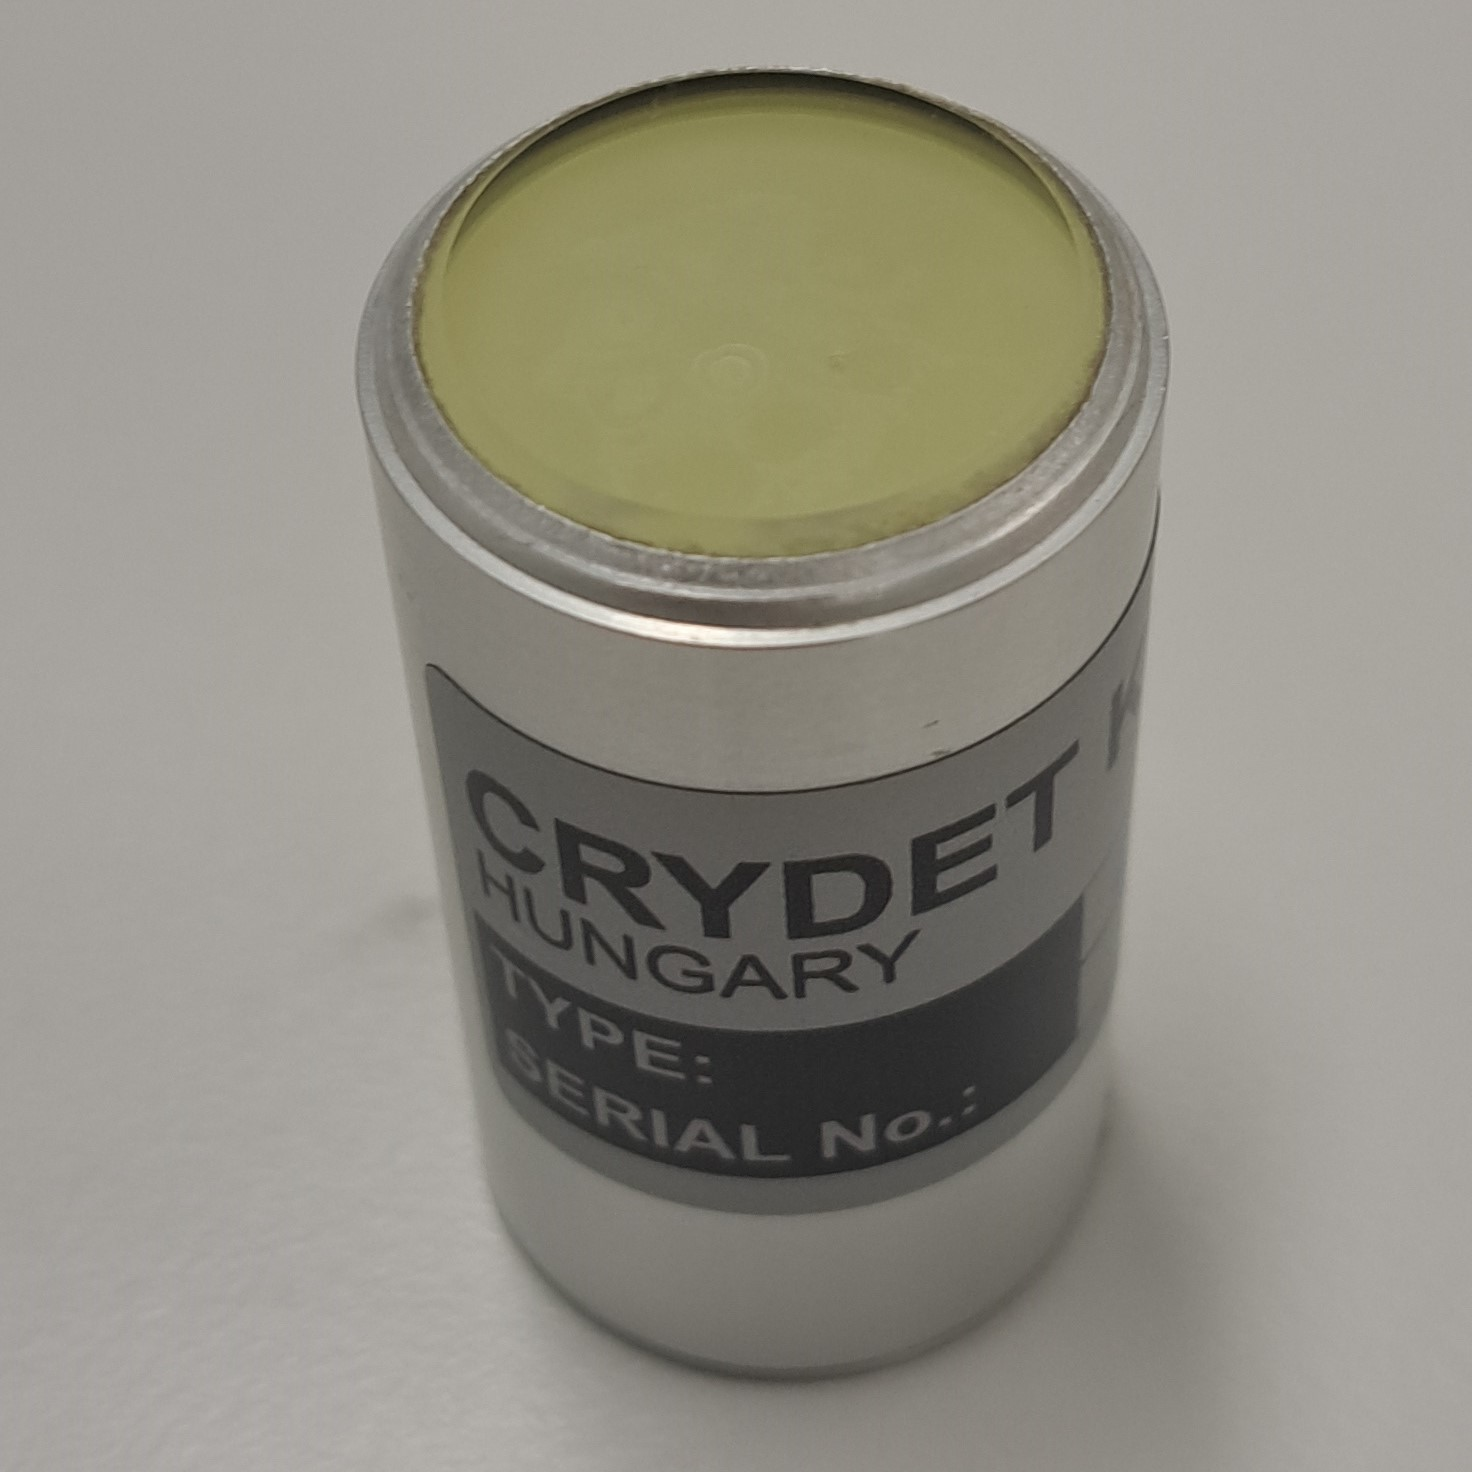
\includegraphics[width=0.7\textwidth]{photo/Crystal.jpg}

        \caption[Photo d'un cristal NaI]{Photo d'un cristal NaI doper au thallium. Dimension~: diamètre 28*50~mm}
        \label{fig_Nai}
    \end{subfigure}
    \begin{subfigure}[t]{0.5\textwidth}
        \centering
        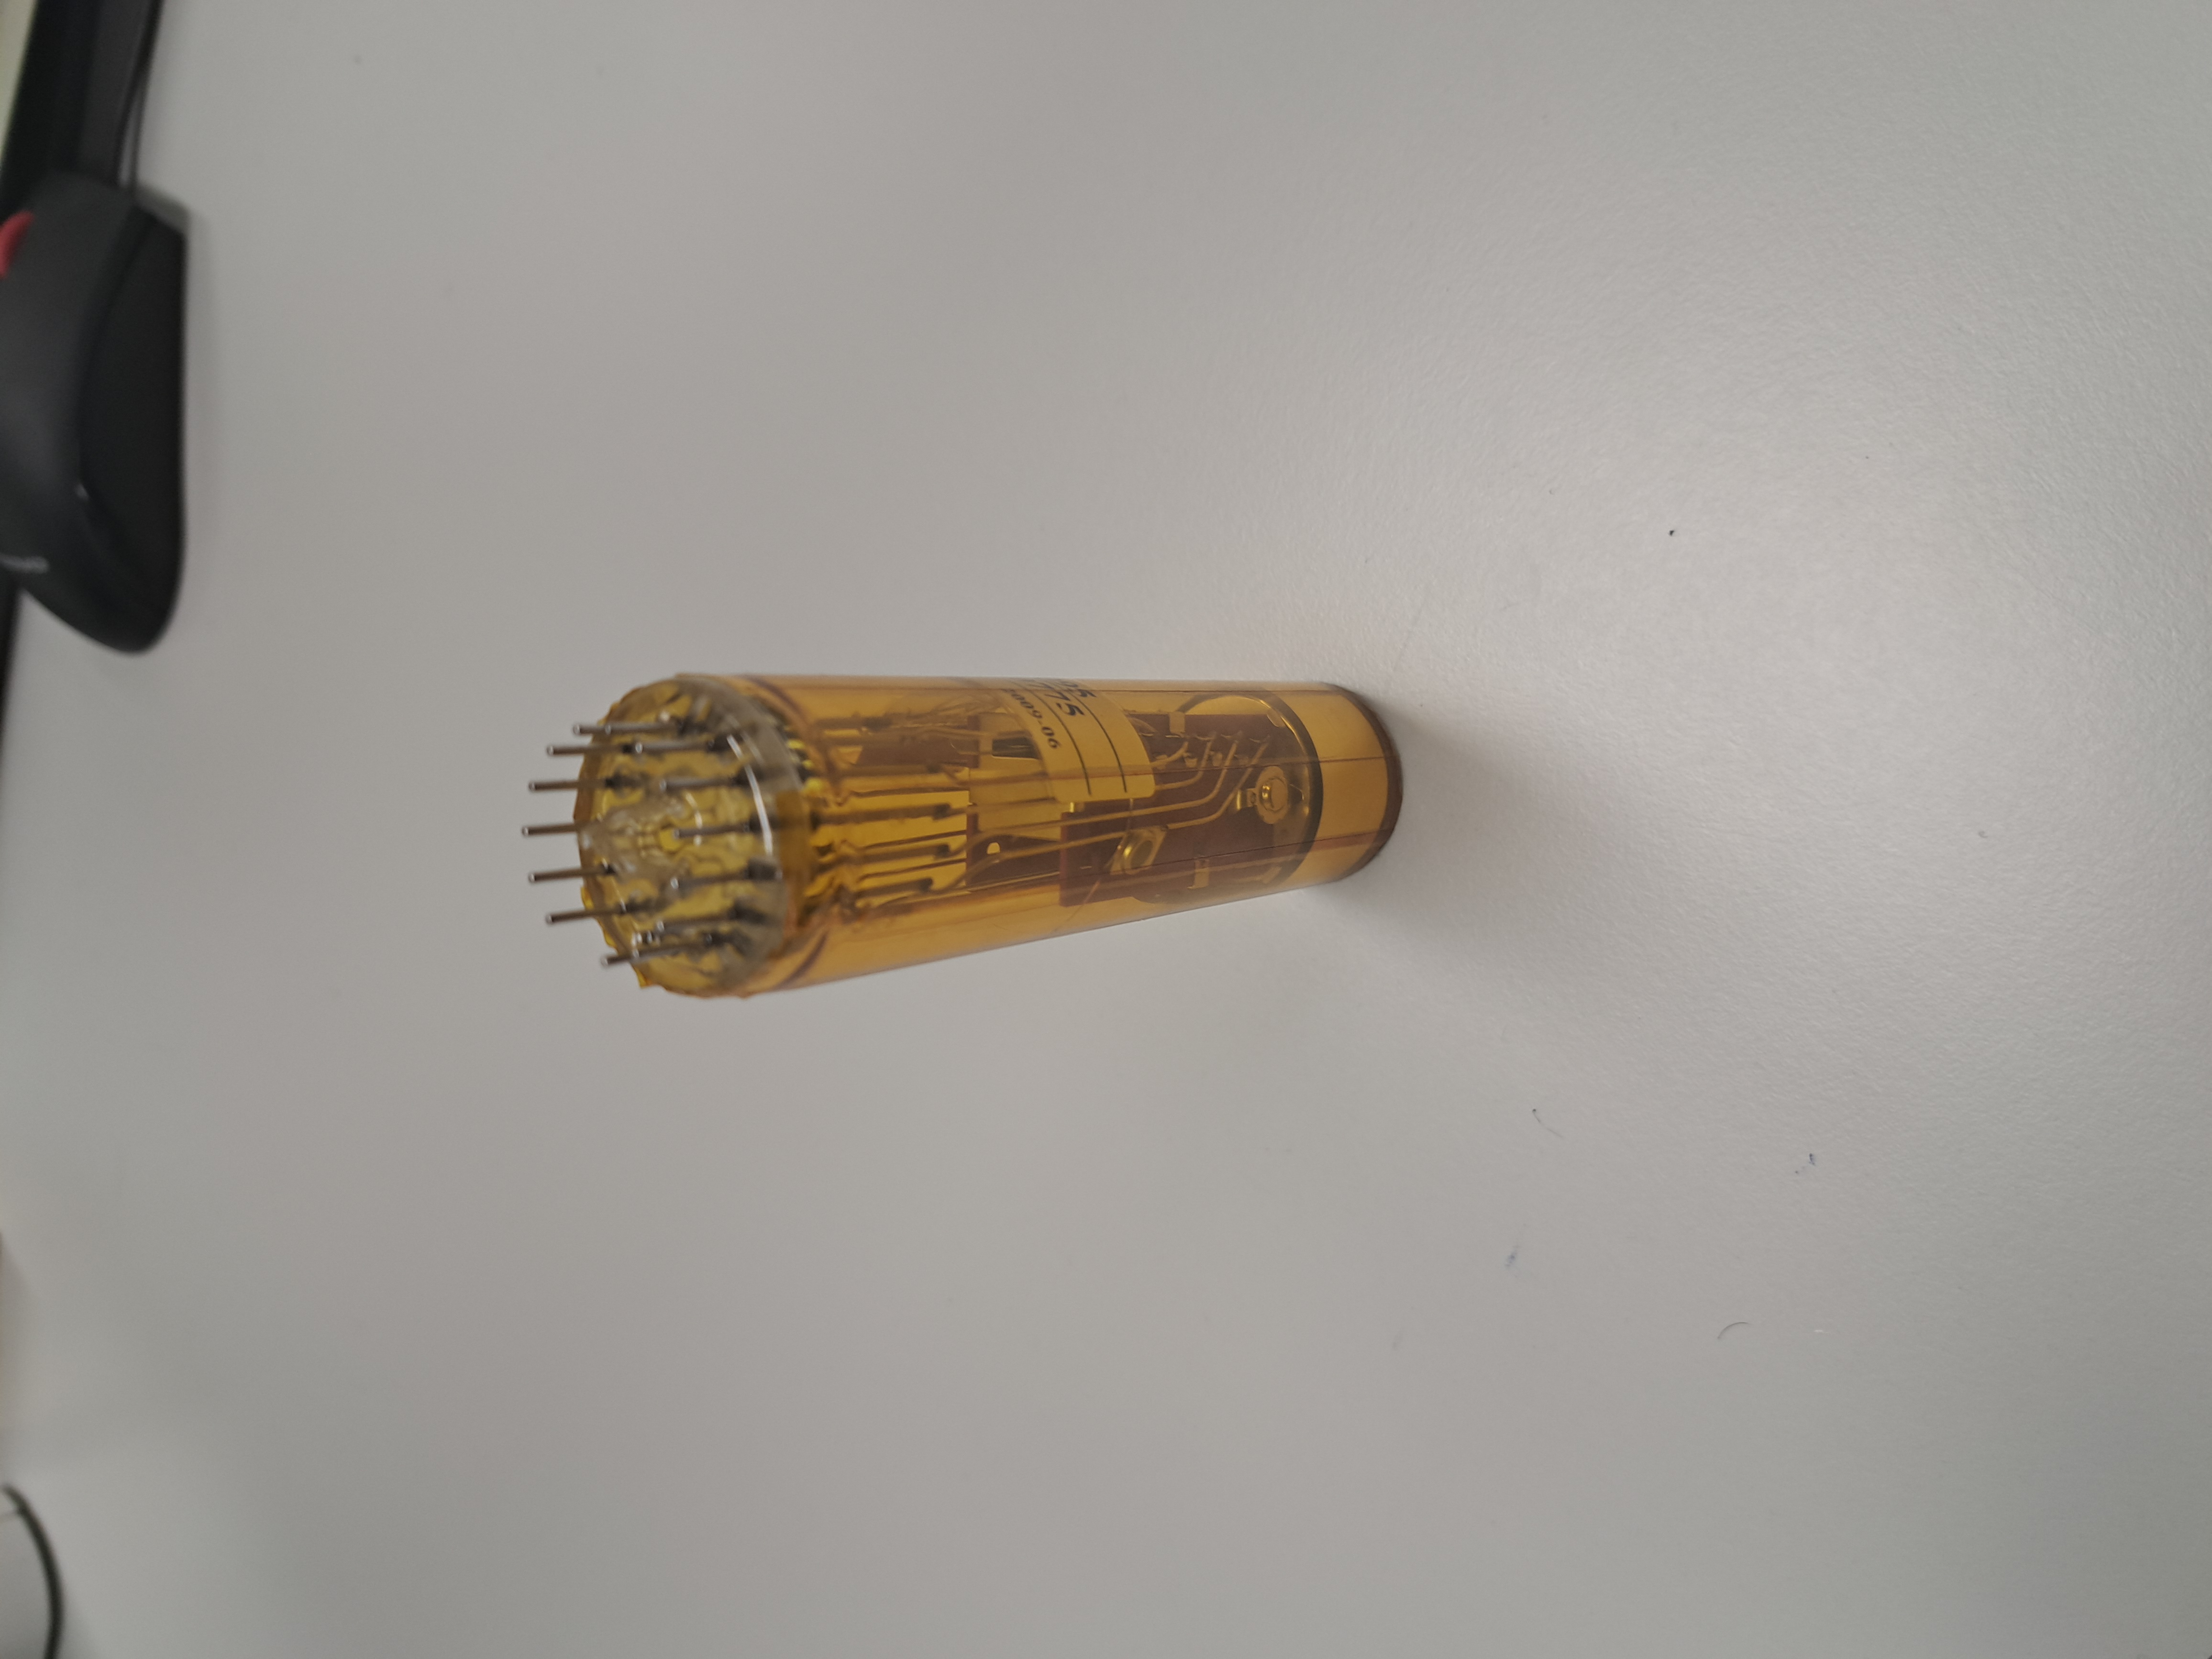
\includegraphics[width=0.7\textwidth]{photo/PMT.jpg}

        \caption[Photo d'un tube photomultiplicateur]{Photo d'un tube photomultiplicateur. Noter la fêlure à gauche de l'étiquette. Dimension~: diamètre 29*114~mm}
        \label{fig_PMT}
    \end{subfigure}
    \caption{Fonctionement d'une sonde gamma}

\end{figure}
\begin{description}
    \item[Un cristal NaI(Th)] C'est un cristal former de sodium et d'idode avec quelque atome de thallium repartie dans sa stucture cristaline. Quand un photon vient frapper un atome du crystal il vas devenir ionizer due a la grand energy du photon. En se desexitant, les atome doive repasser par des niveau d'energie et donc l'energie qu'il dissipe a travers une emission de photon doit avoir une energie precis qui ce traduit par une longeur d'onde dans le visible. Nous avont donc un outil capable de transformer un rayonement haut energie en quelque chose avec moins d'energie que nous savons mesurer. (voir partie gauche de la \cref{fig_detecteur_gamma,fig_Nai})~\cite{site:explication_NaI}
        \item[Un tube photomultiplicateur]ce tube permet de convertir un photon en un photoélectron qui est ensuite multiplié par le tube pour être converti en signaux électriques. Pour cela quand un photon vient du cristal NaI il impact une photocathode qui eject un electon due a l'effet photoelectrique. Les electon resultant sont ensuite aceler vers le premier dynode car elle a un potentielle $\sim$ 100~V. Comme il acceler, il gagne de l'energie et quand il frappe la dyanode, elle vas relaccher plusieur electron de plus basse energie. Ces photon vont ensuit etre acceler par le prochain echellon qui est lui aussi tenu a un potentielle de $\sim$ 100~V par rapport a l'etape d'avant. Si chaque echelon mutltiplie par 4 et qu'il y a 12 etape, notre gain serait de $4^{12}\approx10^{7}$. L'utilisation d'un PMT implique d'avoir un generateur haut tention car le photocathode seras maintenu a $\sim-1200$~V, il faut une atmosphere protectrice ou que le vide soit fait dans le tube et qu'il soit proteger de champs magnetique car il pourait devier les electon des dyanode et ainsi reduire le gain du tube. (Voir partie droite de la \cref{fig_detecteur_gamma,fig_PMT})~\cite{book:photomultiplier_tube}
\end{description}

À la demande du client (Somaïr), une sonde basse a été incluse dans le projet en plus de la sonde haut prevue initialement pour permettre de faire des mesures aux niveaux du sol comme elle était faite avant (voir \cref{ssec_extraction,fig_AP_geiger}). %photo et section
Les études internes montrent que les mesures les plus fiables sont faites à partir de la sonde haute donc la décision a été prise d'inclure les deux. À l'heure actuel, selon les données enregistrées par la sonde, 68,5~\% des mesures sont faits à partir de la sonde haute et 29~\% à partir de la sonde basse. Les autres mesures sont faites avec une combinaison des deux.

\subsection{Le GPS différentiel}
\label{ssec_Gps_differenciel}
Pour que la CanOp puisse fonctionner correctement, il faut qu'elle soit située très précisément ($\pm$ 10~cm sur les axes x et y et $\pm$ 1~cm sur les axes z), or un GPS classique n'arrive qu’a atteindre $\pm$~3~m horizontalement et $\pm$ 5~m verticalement \cite{GPS_accuracy} dus notamment aux perturbations atmosphériques que subisse les signaux.
\begin{figure}

    \begin{subfigure}[t]{0.5\textwidth}
        \centering
        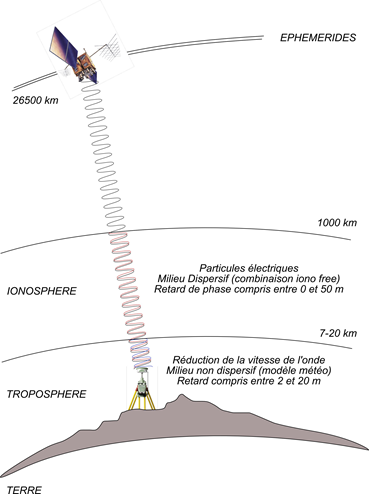
\includegraphics[height=0.9\textwidth]{she/GPS-mode-Naturel-5-10m.png}

        \caption[Source d'erreur des GPS]{Schéma présentant les sources d'erreur des GPS. Source~: Orphéon}
        \label{fig_GPS_error_source}
    \end{subfigure}
    \begin{subfigure}[t]{0.5\textwidth}
        \centering
        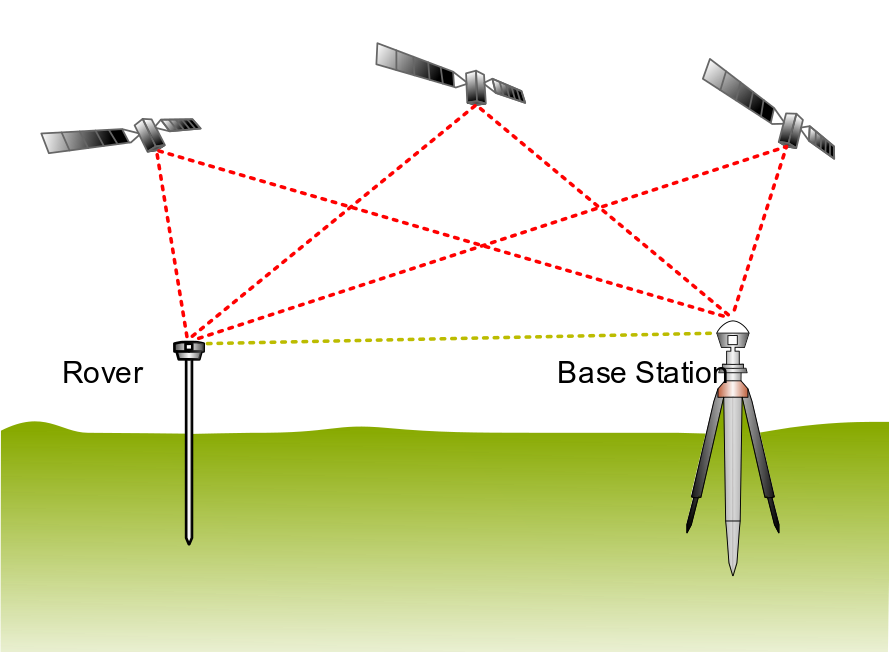
\includegraphics[width=0.9\textwidth]{she/Real_time_kinematic.png}

        \caption[Shema d'un systeme GPS differenciel]{Schéma d'un système GPS différentiel. Source~: \href{https://commons.wikimedia.org/wiki/File:Real_time_kinematic.svg}{TS Eriksson}, \href{https://creativecommons.org/licenses/by-sa/4.0}{CC BY-SA~4.0}, via Wikimedia Commons}
        \label{fig_RTK}
    \end{subfigure}
    \caption{Erreur du GPS et fonctionnement GPS RTK}
\end{figure}

Une des solutions possibles pour contourner ces problèmes est d'utiliser un GPS différentiel. Le principe de fonctionnement est$ sim$ple, une station fixe à proximité de notre zone de mesure reçoit également les signaux GPS et en connaissant sa position précise peuvent calculer et transmettre les corrections nécessaires. \cite{site:GPS_diff}

\subsection{L'électronique}

L'électronique de la CanOp est ce qui permet a tout de fonctioner ensemble. Cette electronique est composé de deux PCB:
\begin{itemize}
    \item Un PCB pour la batterie et le bouton pousoire
    \item Un PCB pour le GPS, les sondes et la communication bluetooth avec la tablette
\end{itemize}

L'operateur interagit avec avec la sonde que grace a un bonton pousoire qui peut lui donner du feed back sur l'etat de la sonde a travers deux LED integrer au bouton. Les donner issue des sondes sont juste des pulses de courant que le secound PCB convertit en signal numerique. c'est donner sont ensuite aggreger avec les donner du GPS qui sont transmit avec un conection RS-232. Les donnée sont ensuit renvoyé par ce bus au module du GPS qui contient le module bluetooth qui permet de communiquer avec la tablette. Le Gps est connecter avec sont un conecteur 7 broche qui est multifonction. Si 'lon debranche le GPS, on peut utiliser ce connecter pour charger la battery interne de la sonde. Il existe egalement un dongle bluetooth qui peut si conecter pour perrmetre l'interfacage avec la sonde si le module GPS est indisponible. Les deux PCB sont contenu dans leur moitier de la sonde et sont entreconecter garce a un connecteur 7 broche. Par mesure de securiter, le fil positif de la batterie fait un aller retour sur le connecteur entre les deux partie de la sondes pour que l'alimentation soit automatiquement couper si on separt les deux partie de la sonde.